\chapter{Design del sistema}

\section{Introduzione}
In questo documento mostreremo delle soluzioni concrete per il modello di analisi effettuato nel documento di \docref{cha:analisi}, aggiungeremo quindi il \emph{come} al \emph{cosa}. Mostreremo quindi una specifica architetture del sistema e aggiungeremo il necessario per rendere possibile l'implementazione dei requisiti formalizzati nel documento di \docref{cha:specifica_requisiti}.

\section{Architettura del sistema}
Vengono di seguito mostrate l'architettura fisica e quella software del sistema.

\subsection{Architettura fisica}
L'architettura fisica del sistema è mostrata dalla seguente figura:
\begin{center}
   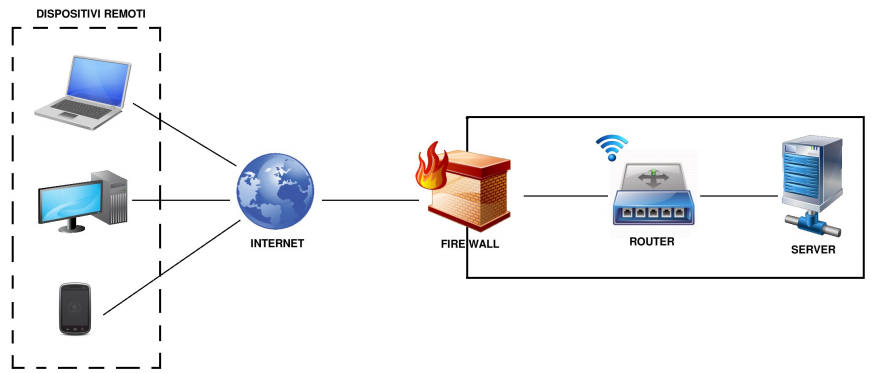
\includegraphics[width=\textwidth]{assets/architetturaFisica}
\end{center}

\subsection{Architettura software}
L'architettura software del sistema è mostrata dalla seguente figura:
\begin{center}
   \includegraphics[width=\textwidth]{assets/architetturaSoftware}
\end{center}

\section{CMS}
Per realizzare il sistema finora descritto utilizzeremo il \gls{cms} commerciale WordPress, scelto in quanto dispone di una grande quantità di plugin per soddisfare tutte le funzionalità precedentemente descritte. Questo sarà installato nel server e si occuperà della comunicazione con i fruitori del servizio e integrerà il database.

\subsection{Installazione}
Per installare WordPress sarà necessario seguire i seguenti passi:
\begin{enumerate}
	\item Scaricare e decomprimere il pacchetto di WordPress;
	\item Creare un database per WordPress sul server web, ed un utente MySQL che abbia tutti i permessi per accederci e modificarlo;
	\item Rinominare il file \texttt{wp-config-sample.php} in \texttt{wp-config.php};
	\item Aprire \texttt{wp-config.php} in un editor di testo e inserire i dettagli del database;
	\item Caricare i file di WordPress nella cartella principale del server web;
	\item Lanciare lo script di installazione di WordPress visitando la pagina \texttt{http://esempio.com/wp-admin/install.php};
\end{enumerate}

\subsection{Configurazione}
-abilitare iscrizione e login
-grafico per fare la grafica
-creazione delle pagine necessarie atraverso la console admin



\subsection{Plugin}
WordPress mette a disposizione oltre 47mila plugin, i quali estendono ed espandono le funzionalità di base presenti.
L'installazione e l'attivazione dei plugin è immediata, in quanto è possibile effettuarla direttamente tramite il pannello di controllo di WordPress.
Per implementare tutte le funzionalità precedentemente descritte sarà necessario installare ed attivare i seguenti plugin.


) advanced acces manager - ruoli
) wp user manager - gestione profili
) wp user fronted - modifica campi proprio profilo dal frontend
) Dokan- vetrine e pagine prodotti e gestione "negozi privati", ricerca,
) buddypress con plugin follow/unfollow - follow/unfollow
) WP Support Plus Responsive Ticket System  - gestione ticket
) wp Report Post - report dei contenuti inappropriati e segnalazioni
) Ninja Forms - gestione forms per iscrizioni e cose varie


Managing your members, creating front-end profiles and custom login and registration pages should be easy. With this plugin, it finally is.
WP User Manager lets you create highly customizable user profiles. You easily add custom user registration, login and password recovery forms to your WordPress website. WP User Manager is the best solution to manage your users.

\subsubsection{User Role Editor}
 \paragraph{Descrizione.} Con il plugin \gls{ure} è possibile cambiare le capacità del ruolo utente semplicemente. Basta spuntare le caselle di controllo delle capacità che si desidera aggiungere al ruolo selezionato. Aggiungere nuovi ruoli e personalizzarne le capacità in base alle proprie esigenze. Il ruolo creato automaticamente può essere eliminato se non ci sono utenti a cui tale ruolo è assegnato. Anche il ruolo assegnato di default alla creazione di ogni nuovo utente può essere modificato. Le capacità possono essere assegnate sulla base del singolo utente. Ruoli multipli possono essere assegnati all'utente simultaneamente. È possibile aggiungere nuove funzionalità e rimuovere le funzionalità non necessarie che potrebbero essere state lasciate da un plugin disinstallato.
 \paragraph{Utilizzo.}  \gls{ure} potrà essere utilizzato dall'amministratore per la gestione dei ruoli, dei profili, degli account e dell'assegnamento dei privilegi in base a quali ruoli un account possiede.
 \paragraph{Configurazione.} Si dovranno creare i ruoli Visitatore, Utente, Produttore, Assistente, Redattore, Moderatore e Amministratore, assegnando ad ognuno i corrispettivi privilegi.

\subsubsection{WP User Manager}
\paragraph{Descrizione.} Il plugin \gls{wpum} permette di creare profili altamente personalizzabili, è possibile inoltre personalizzare il form di iscrizione, login e recupero password. 
\paragraph{Utilizzo.}  \gls{wpum} verrà utilizzato per creare i profili utente e produttore.
\paragraph{Configurazione.}  Si dovranno creare i profili descritti e associarli agli account in base al loro ruolo.


\subsubsection{WP User Frontend}
\paragraph{Descrizione.} Questo plugin fornisce alle persone autenticate la possibilità di creare nuovi post, di modificare i propri profili direttamente dal fronted, senza dover accedere al pannello di amministrazione.
\paragraph{Utilizzo.}  \gls{wpuf} potrà essere utilizzato dall'amministratore per fornire alle persone autenticate la possibilità di modificare i propri profili direttamente dal fronted.
\paragraph{Configurazione.} Si dovrà dare alle persone iscritte la possibilità di personalizzare il profilo in base al ruolo posseduto.

\subsubsection{WooCommerce}
\paragraph{Descrizione.} \gls{wc} è un plugin per e-commerce gratuito che ti permette di vendere in maniera ottimale qualsiasi cosa. \gls{wc}fornisce sia ai proprietari che agli sviluppatori il controllo completo del proprio shop.
\paragraph{Utilizzo.} \gls{wc} potrà essere utilizzato per gestire la vetrina e l'inserimento e la modifica di prodotti, recensioni ad essi associate, commenti a recensioni, valutazioni e giudizi.
\paragraph{Configurazione.} Si dovrà configurare \gls{wc} in modo da non permettere la vendita di prodotti, ma solo la loro esposizione.

\subsubsection{WC Vendors}
\paragraph{Descrizione.} Questo plugin permette di creare il proprio marketplace e di fornire ai venditori la possibilità di vendere come su etsy, Envato, eBay, o Amazon. \gls{wcv} permette a più venditori di vendere i propri prodotti.
\paragraph{Utilizzo.} \gls{wcv} potrà essere utilizzato per gestire più vetrine contemporaneamente, permettendo ad ogni produttore di avere la propria vetrina in cui mostrare i propri prodotti.
\paragraph{Configurazione.} Si dovrà configurare \gls{wcv} in modo da non permettere la vendita di prodotti, ma solo la loro esposizione.

\subsubsection{BuddyPress}
\paragraph{Descrizione.}
BuddyPress è una insieme di componenti comuni a un tipico social network, e permette di aggiungere molte funzionalità attraverso l'esteso sistema di plugin di WordPress.
BuddyPress è focalizzato sulla facilità di integrazione, facilità d'uso e estensibilità. È un software per creare social network volutamente potente anche se incredibilmente semplice, costruito dai contributori di WordPress.
Consenti ai membri di registrarsi per aprire un profilo, avere conversazioni private, effettuare collegamenti, creare per interagire nei gruppi, e molto altro. 
\paragraph{Utilizzo.}
\gls{bp} verrà utilizzato per gestire il lato social del sistema, oltre a gestire le richieste dagli utenti ai produttori.
\paragraph{Configurazione.}
Per configurare BuddyPress e gestire il sistema di follower/followed è necessario installare il plugin \gls{bpf}

\subsubsection{BuddyPress Follow}
\paragraph{Descrizione.}
Questo plugin permette di estendere le funzionalità di \gls{bp} per implementare il sistema di follower/followed .
\paragraph{Utilizzo.} Verrà utilizzato per implementare il sistema di follower/followed.
\paragraph{Configurazione.} Non necessita di configurazione.

\subsubsection{WP Support Plus Responsive Ticket System}
\paragraph{Descrizione.}
\paragraph{Utilizzo.}
\paragraph{Configurazione.}

\subsubsection{WP Report Post}
\paragraph{Descrizione.}
\paragraph{Utilizzo.}
\paragraph{Configurazione.}

\subsubsection{Ninja Forms}
\paragraph{Descrizione.}
\paragraph{Utilizzo.}
\paragraph{Configurazione.}